\chapter{背景知識}

\section{Refactoring}
\indent
Refactoring\cite{RefactoringBook}通常被定義為「在不改變程式碼外在行為的前提下,改善既有程式碼內部架構的過程」,當專案越加龐大時,內部程式碼的架構將會因為不同的需求而產生不一樣的設計,時間久了就會使專案程式碼越來越不可讀甚至難以擴充,在此種狀況下,為了提升程式碼的品質,儘管程式能夠正常運作,仍然需要為其重構,在開發人員確保程式行為一致的前提下,調整內部的設計,以此達到重構的目的。

\indent
重構測試程式碼與重構一般程式碼也有所不同,在重構一般程式碼時,會著重在內部架構的設計,讓其未來被使用及維護上都更加地容易,並且重構後可以透過單元測試檢查該次重構是否正確;而重構測試程式碼時,則是根據每個測試當下的狀況,判斷其設計是否符合當時所需來進行調整,或是改變測試的順序讓整體運作上能夠更加地順暢,重構完成後可以再次執行與該次重構相關的測試,確認其與重構前的行為是一致的。儘管兩者有不同之處,但其最終目的皆是希望讓整體程式碼的設計更加完善,進而提升程式碼的品質。

%\indent
%Refactoring\cite{RefactoringBook}通常被定義為「在不改變程式碼外在行為的前提下,改善既有程式碼內部架構的過程」,在過程中,不針對既有的錯誤進行修改,也不新增額外的功能,完全只專注於改善程式碼的內部設計,提高整體程式的品質,使其未來被使用及維護上都更加地容易。
%
%\indent
%Refactoring: Improving the Design of Existing Code\cite{RefactoringBook}一書中有介紹常用的重構方法,其中包含較簡單的重構方法,例如:重新命名變數、函數、移動函數等等,以及較複雜的重構方法,例如:將程序設計轉化為物件設計。程式開發人員能夠利用這些已知的方法,針對其需要改善的程式碼進行重構,讓重構過程能夠更加順利且容易,進而提高整體內部設計的品質。

\section{Robot Framework}\label{s2.2}
\indent
Robot Framework是一個基於Python\cite{python}所開源的自動化框架,通常被使用於開發驗收測試及驗收測試驅動開發(Acceptance test-driven development)\cite{ATDD}、行為驅動開發(Behavior-driven development)\cite{BDD}。由於關鍵字驅動測試(Keyword-driven testing)\cite{robotframework}的特色,開發人員能夠使用簡單且較容易理解的關鍵字撰寫測試腳本,讓整體具備極高的可讀性及降低開發的門檻,並且開發人員能夠將多個關鍵字包裝成更高階的關鍵字,使測試腳本閱讀起來更加地接近自然語言。

\indent
Robot Framework同時也擁有極佳的可擴充性,除了能夠使用官方及外部函式庫所提供的關鍵字以外,當開發人員遭遇現有關鍵字無法滿足開發需求時,也能夠透過Python或Java自行擴充所需的函式庫,滿足新關鍵字的需求。此外Robot Framework提供了公開的API(Application Programming Interface)\cite{RobotFrameworkAPI},例如:針對現有的測試腳本進行解析、調整測試腳本執行的結果等等,讓開發人員能夠依照需求自行製作其他的功能,使設計測試腳本的過程能夠更加彈性。程式碼\ref{l2.1}為Robot Framework 測試腳本之實例

\begin{lstlisting}[caption=Robot Framework 實例腳本, label={l2.1}]
*** Settings ***
Library     SeleniumLibrary
Resource    ../microsoft.txt

Test Setup    Go To English Microsoft

*** Variables ***
@{welcomeTaipei} =    Welcome    To    Taipei

*** Test Cases ***
Go To "Windows Security" Page And Log Welcome Text
    Go To Windows Page
    Open Windows 10 Menu
    Go To "Windows Security" Page
    "Windows Security" Page Should Be Visible
    FOR    ${var}    IN    @{welcomeTaipei}
        Log Double Text    ${var}
    END
    [Teardown]    Close Browser
    
*** Keywords ***
Go To English Microsoft 
    Go To Microsoft
    Open Language Option
    Select English Language
\end{lstlisting}

\section{抽象語法樹}\label{s2.3}
\indent
抽象語法樹(Abstract Syntax Trees)\cite{AST}是程式碼結構的一種抽象表達,利用樹狀結構展現出程式中的語法關係,每個節點分別表示程式碼中的一種結構,但不會將語法中的細節完全呈現,例如:Java中利用括號所表示的領域區分,在節點中並不會被呈現、條件式判斷則以節點下的分支進行表示,並非表示在節點之中。

\indent
在Python中,開發人員能夠透過AST套件\cite{ASTmodule}開發與抽象語法樹相關的程式碼,對於當前程式碼在語法層面的操作及檢視都提供了十分大的幫助。套件中提供了parse相關的輔助函數,可以讓開發人員更簡單地取得所需的語法樹,此外也提供了方便開發人員訪問各節點的可繼承類別,例如:NodeVisitor、NodeTransformer,讓開發人員能夠依照需求,自行新增含有不同功能的類別,運用上擁有較大的彈性。當其運用在Robot Framework上時,其可搭配Robot Framework提供的公開API,將測試檔案解析成抽象語法樹(AST)模型,讓開發人員在對於測試腳本及測試資源的存取上都更加地簡單。


%\subsection{抽象語法樹應用於Robot Framework}\label{s2.3.2}
%\indent
%Robot Framework提供了公開的API,其可將測試檔案解析成抽象語法樹(AST)模型,搭配Python中AST套件,讓開發人員在對於測試腳本及測試資源的存取上都更加地簡單。因此開發人員能夠調整Robot Framework API的使用方法,且使用繼承AST套件中訪問節點功能及含有其他需求功能的類別,以此達成不同需求中的目的,使整體有較廣泛的運用。

%\begin{lstlisting}[caption=解析測試腳本實例, label={l2.3}]
%import ast
%from robot.api import get_model
%
%
%class TestCaseNamePrinter(ast.NodeVisitor):
%
%    def visit_File(self, node):
%        print('File ' + node.source + ' has following tests:')
%        self.generic_visit(node)
%    
%    def visit_TestCaseName(self, node):
%        print(f"- {node.name} on line {node.lineno}")
%
%model = get_model('example.robot')
%printer = TestCaseNamePrinter()
%printer.visit(model)
%\end{lstlisting}
%
%\begin{figure}[H]
%    \centering
%    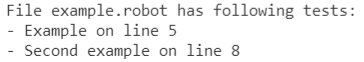
\includegraphics[width=0.7\textwidth]{picture/parsing_example_2.PNG}
%    \caption{解析測試腳本實例結果}
%    \label{f2.5}
%\end{figure}

\section{Eclipse}\label{s2.4}
\indent
團隊開發測試腳本所使用之整合式開發環境(RED)是基於Eclipse所開發出來的,而Eclipse\cite{Eclipse}是一個跨平台的開源整合式開發環境,起初是以開發Java作為主要目的,後續透過外掛程式的擴展,可使其成為其他語言的開發工具,例如:C++、PHP、Python等等。Eclipse僅以圖形API、Java開發環境、外掛程式開發環境等作為基礎核心,其餘功能則一律以外掛程式的方式附加於核心之上,例如:圖形編輯器、複雜重構、版本控制等等功能。

\indent
由於Eclipse除了核心以外,其餘皆為外掛程式,使其具有良好的擴充性,更重要的是,平台定義了十分明確的機制,讓不同的外掛程式可以利用延伸點(extension points)及貢獻(contribute)相互合作,既存的功能能夠被新功能使用,而新功能也可以輕鬆地整合於平台之中。圖\ref{f2.6}為Eclipse平台之架構\cite{EclipseStructure}

\begin{figure}[H]
    \centering
    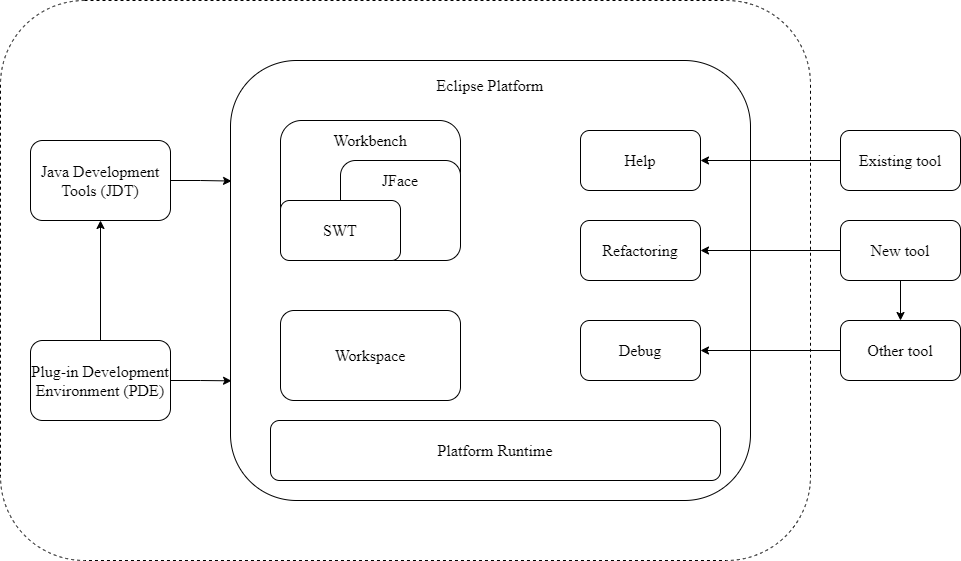
\includegraphics[width=0.8\textwidth]{picture/eclipse_structure.png}
    \caption{Eclipse外掛式架構\cite{EclipseStructure}}
    \label{f2.6}
\end{figure}

\newpage
\section{Jython}
\indent
Jython\cite{Jython}是一個利用Java所撰寫的Python直譯器,在任何支援JVM\cite{JVM}(Java virtual machine)的環境上皆可使用,也代表著能夠使用JVM中的Java函式庫。Jython提供開發人員在開發過程中能夠自由地混用Java及Python兩種不同的語言,使開發能夠更加地彈性。

\begin{lstlisting}[caption=Jython於Python語言環境中執行Java之實例, label={l2.4}]
from java.lang import System

current_java_version = System.getProperty('java.version')
strInPython = "Current java version is " + current_java_version
System.out.println(strInPython)
\end{lstlisting}

\begin{lstlisting}[caption=Jython於Java語言環境中執行Python之實例, label={l2.5}]
import org.python.util.PythonInterPreter;

public class RunPythonInJava{
    public static void main(String []args){
        PythonInterPreter pyRunner = new PythonInterPreter();
		pyRunner.exec("print('I am from python world!')");
	}
}
\end{lstlisting}